% -*- root: ../main.tex -*-
\chapter{Design di Dettaglio}
\section{ECS}
 %giustificazione ecs
 %Ogni sistema si occupa di gestire solamente uno o più componenti, aggiornandoli in blocco contemporaneamente. Questo approccio, in contrasto con l'approccio più OOP che consisterebbe nel modellare ogni entità come un oggetto, che deve implementare una sotto-interfaccia diversa in base al tipo, ereditando i metodi per l'aggiornamento. Questo causa problemi di performance all'aumentare delle entità da gestire, infatti ad ogni aggiornamento sarà caricato in cache l'intero oggetto e andrà recuperato dalla virtual table(TODO CHECK THIS) il metodo relativo all'aggiornamento. Ciò comporta un degradamento importante delle performance dato che gli accessi in RAM sono molto più lenti di quelli direttamente in cache. Sfruttando l'approccio ECS invece è possibile sfruttare meglio la cache, in quanto per ogni aggiornamento i componenti vengono caricati cache in blocco e processati dallo stesso metodo. 
 \subsubsection{Interazione tra Engine ECS e controller}
 Come spiegato nel \ref{ecs}, i vari gestori di componenti che compongono l'ECS sono coordinati tra di loro tramite un coordinator. Esso fa da punto di contatto con l'engine vero e proprio esponendo il metofo update
 \begin{figure}[H]
	\centering
	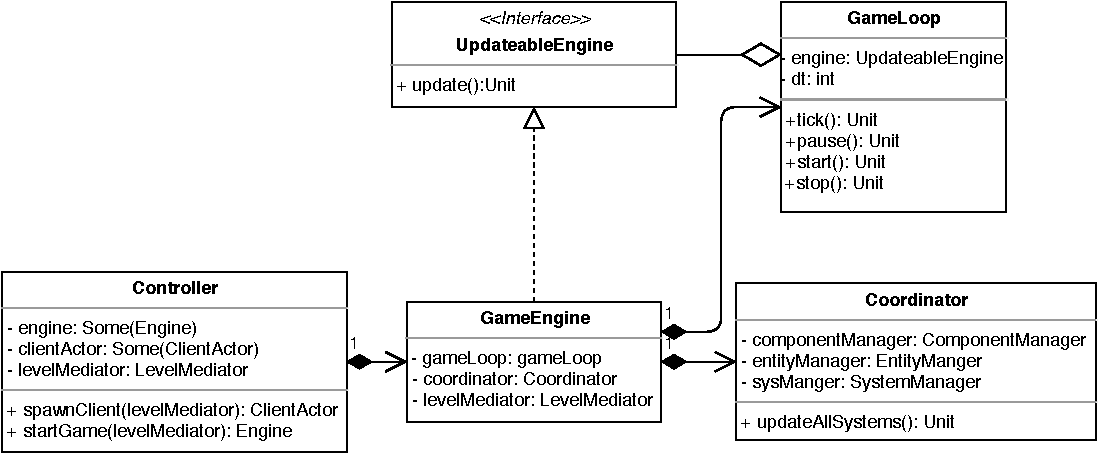
\includegraphics[width=\columnwidth]{drawio/ECS-engine-controller/ecs-engine-controller.pdf}
	\caption{Diagramma raffigurante ecs, engine e controller e le loro interazioni.}
	\label{fig:ecsenginecontroller}
\end{figure}
 \section{View}
 \section{File manager}
 \section{Audio manager}
 \section{Engine}
 \section{Client-Server}
\section{Scelte Rilevanti}
\section{Pattern di Progettazione%design???????
}
\subsection{Mediator}
\section{Organizzazione del Codice}
/src